%\documentclass[10pt,notes]{beamer}       % print frame + notes
%\documentclass[10pt, notes=only]{beamer}   % only notes
\documentclass[11pt]{beamer}              % only frames

%%%%%% IF YOU WOULD LIKE TO CREATE LECTURE NOTES COMMENT OUT THE FOlLOWING TWO LINES
%\usepackage{pgfpages}
%\setbeameroption{show notes on second screen=bottom} % Both

\usepackage{graphicx}
\DeclareGraphicsExtensions{.pdf,.png,.jpg}
\usepackage{color}
\usetheme{winslab}
\usepackage[utf8]{inputenc}
\usepackage[english]{babel}
\usepackage{amsmath}
\usepackage{amsfonts}
\usepackage{amssymb}




\usepackage{algorithm2e,algorithmicx,algpseudocode}
\algnewcommand\Input{\item[\textbf{Input:}]}%
\algnewcommand\Output{\item[\textbf{Output:}]}%
\newcommand\tab[1][1cm]{\hspace*{#1}}

\algnewcommand{\Implement}[2]{\item[\textbf{Implements:}] #1 \textbf{Instance}: #2}%
\algnewcommand{\Use}[2]{\item[\textbf{Uses:}] #1 \textbf{Instance}: #2}%
\algnewcommand{\Trigger}[1]{\Statex{\textbf{Trigger:} (#1)}}%
\algnewcommand{\Events}[1]{\item[\textbf{Events:}] #1}%
\algnewcommand{\Need}[1]{\item[\textbf{Needs:}] #1}%
\algnewcommand{\Event}[2]{\Statex \item[\textbf{On#1:}](#2) \textbf{do}}%
\algnewcommand{\Trig}[3]{\State \textbf{Trigger}  #1.#2 (#3) }%
\def\true{\textbf{T}}
\def\false{\textbf{F}}


\author[Furkan Küçük]{Furkan Küçük\\\href{mailto:kucuk.furkan@metu.edu.tr}{kucuk.furkan@metu.edu.tr}}
%\author[J.\,Doe \& J.\,Doe]
%{%
%  \texorpdfstring{
%    \begin{columns}%[onlytextwidth]
%      \column{.45\linewidth}
%      \centering
%      John Doe\\
%      \href{mailto:john@example.com}{john@example.com}
%      \column{.45\linewidth}
%      \centering
%      Jane Doe\\
%      \href{mailto:jane.doe@example.com}{jane.doe@example.com}
%    \end{columns}
%  }
%  {John Doe \& Jane Doe}
%}

\title[]{OLSR Algorithm Presentation}
\subtitle[Short SubTitle]{The algorithm that will change the world}
%\date{} 

\begin{document}

\begin{frame}[plain]
\titlepage
\note{In this talk, I will present .... Please answer the following questions:
\begin{enumerate}
\item Why are you giving presentation?
\item What is your desired outcome?
\item What does the audience already know  about your topic?
\item What are their interests?
\item What are key points?
\end{enumerate}
}
\end{frame}

\begin{frame}[label=toc]
    \frametitle{Outline of the Presentation}
    \tableofcontents[subsubsectionstyle=hide]
\note{ The possible outline of a talk can be as follows.
\begin{enumerate}
\item Outline 
\item Problem and background
\item Design and methods
\item Major findings
\item Conclusion and recommendations 
\end{enumerate} Please select meaningful section headings that represent the content rather than generic terms such as ``the problem''. Employ top-down structure: from general to more specific.
}
\end{frame}
%
%\part{This the First Part of the Presentation}
%\begin{frame}
%        \partpage
%\end{frame}
%
\section{The Problem}
%\begin{frame}
%        \sectionpage
%\end{frame}

\begin{frame}{The problem}
% \framesubtitle{Tell a \alert{STORY} from the background to the conclusion}
\begin{block}{Routing Problem in MANETs} 
    The challenge is to create a routing protocol for mobile ad-hoc networks (MANETs) that adapts in real-time to their constantly changing network topologies, ensuring reliable communication with minimal overhead. Traditional static routing protocols are ineffective in this dynamic environment, which is where the OLSR algorithm comes into play, aiming to resolve these issues.
\end{block}
\note{}
\end{frame}

% \section{The Contribution}
% \begin{frame}
% \frametitle{What is the solution/contribution}
% \framesubtitle{}
% Explain \textbf{YOUR} contributions. Go top-down. Give the brief introduction to the contributions at the beginning of the presentation. A slide should have no more than five to six lines of text or bullets. Prefer figures instead of text: A picture is worth a thousand words.
% \begin{itemize}
% \item Communicate the Key Ideas
% \item Don’t get Bogged Down in Details
% \item Use a Top-down Approach
% \end{itemize}

% The audience will remember at most one single message \textbf{Which message you want to audience to remember? Can you express this message in less than a minute in an elevator?}

% \end{frame}


\section{Motivation/Importance}
\begin{frame}
\frametitle{Motivation/Importance}
% \framesubtitle{``Gain upon solving the problem, pain if not solved'' should be explained}
\textbf{Essential Connectivity:} OLSR addresses the critical need for stable communication in dynamic environments like disaster recovery, military operations, and remote connectivity.

\textbf{Real-world Reflection:} The protocol models our social dynamics, where each node supports and relies on the network, highlighting our interconnected nature.

\textbf{Broad Applications:} From emergency services to smart vehicles, OLSR's efficiency is crucial for the next generation of wireless communication.

\textbf{Complex Balance:} Crafting a protocol that is both adaptive and lightweight in a constantly shifting network topology is a complex yet vital task.
\end{frame}

\section{Background/Model/Definitions/Previous Works}


\subsection{Model, Definitions}

\frame{
\frametitle{Definition of the Problem}
% \framesubtitle{Formal definition of a Stochastic Process}
The routing problem in MANETs that OLSR aims to solve involves determining the most efficient paths for data transmission between mobile nodes in a network where links frequently and unpredictably appear and disappear as nodes move.
}

\subsection{}

\subsection{Background, Previous Works}
\begin{frame}{Background}
    \begin{itemize}
        \item \textbf{DSR (1996, Johnson \& Maltz):} On-demand routing; higher latency compared to OLSR's constant updates.
        \item \textbf{AODV (1999, Perkins \& Royer):} Reactive like DSR; uses routing tables, unlike OLSR's MPRs.
        \item \textbf{DSDV (1994, Perkins \& Bhagwat):} Proactive with full-table broadcasts; OLSR reduces overhead with selective flooding.
        \item \textbf{TORA (1997, Park \& Corson):} Adapts quickly to changes with link reversal; OLSR maintains consistent network topology knowledge.
    \end{itemize}
\end{frame}




\section{Contributions}
% \subsection{Contributions}
\begin{frame}{Contributions}
    \begin{itemize}
        \item \textbf{Proactive Routing:} OLSR provides constant route availability, which is crucial for applications requiring immediate route access.
        \item \textbf{MultiPoint Relays (MPRs):} Reduces the overhead of message flooding by using selected nodes to forward control messages.
        \item \textbf{Optimized Routing Control:} The protocol minimizes control traffic through incremental topology updates rather than full-fledged table exchanges.
        \item \textbf{Topology Dissemination:} OLSR's efficient dissemination of topology information ensures all nodes maintain consistent network knowledge.
        \item \textbf{Scalability:} Designed to scale well in larger networks compared to many other MANET routing protocols.
    \end{itemize}
\end{frame}


\section{Design and Methods}
\subsection{Algorithm Overview}
\begin{frame}
\frametitle{OLSR Algorithm Overview}

The Optimized Link State Routing (OLSR) algorithm involves the following key procedures:

\begin{itemize}
    \item \textbf{Topology Discovery:} Nodes periodically exchange "hello" messages to detect neighbors and assess link status.
    \item \textbf{MPR Selection:} Each node selects a set of neighboring nodes as MultiPoint Relays (MPRs) based on the network topology to efficiently forward messages.
    \item \textbf{Routing Table Calculation:} Nodes use topology information, primarily through MPRs, to calculate the shortest paths to all other nodes in the network.
    \item \textbf{Control Message Flooding:} MPRs disseminate Topology Control (TC) messages across the network, reducing the number of transmissions required to share topology changes.
    \item \textbf{Route Maintenance:} Nodes continuously monitor link status and adapt the network routing tables accordingly, ensuring up-to-date path availability.
\end{itemize}

\end{frame}

\subsection{Algorithm Workflow}
\begin{frame}
    % Add image of OLSR workflow
    \begin{figure}
        \centering
        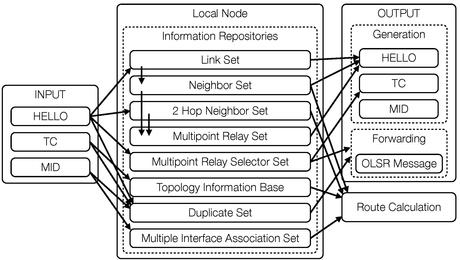
\includegraphics[width=0.8\textwidth]{figures/olsr_overview.jpg}
        \caption{OLSR Algorithm Workflow \cite{wiki:olsr}}
    \end{figure}    
\end{frame}

\subsection{Algorithm Pseudocode}
\begin{frame}
\frametitle{OLSR Algorithm Pseudocode}

\begin{algorithm}[H]
    % \caption{OLSR Algorithm Pseudocode}
    \scriptsize
    \SetKwInput{KwData}{Initialize}
    \SetKwInput{KwResult}{MainLoop}
    \SetKwProg{Fn}{Procedure}{}{}
    
    \KwData{
        \For{each node}{
            Set HelloInterval, TCInterval\;
            Initialize Neighbor Table, Topology Table, Routing Table\;
        }
    }
    
    \KwResult{
        \While{network is operational}{
            Every HelloInterval: BroadcastHelloMessage to neighbors\;
            Every TCInterval: BroadcastTCMessage to MPRs\;
            On receiving a message: Update tables and RecalculateRoutingTable()\;
            MaintainMPRSet based on Neighbor Table\;
        }
    }
    
    \Fn{UpdateTables}{Message}{
        \uIf{Hello message}{
            update Neighbor Table\;
        }
        \ElseIf{TC message}{
            update Topology Table\;
        }
    }
    
    \Fn{RecalculateRoutingTable}{
        Compute shortest path using Topology Table\;
    }
    
    \Fn{MaintainMPRSet}{
        Select minimal set of neighbors covering all two-hop neighbors\;
    }
    
    \end{algorithm}

\end{frame}



\section{Experimental results/Proofs}
\begin{frame}
\frametitle{Experimental Results}
This will be created as the project progresses.
\end{frame}

\section{Conclusions}
\begin{frame}
\frametitle{Conclusions}
This will be created as the project progresses.
\end{frame}

% \subsection{Main Result 1}
% \begin{frame}
% \frametitle{Main Result 1}
% \framesubtitle{}
% Choose \textbf{just the key results}. They should be important, non-trivial, should give the flavour of the rest of the technical details and should be presentable in a relatively short period of time. Use figures instead of tables instead of text.

% Better to present 10\% the entire audience gets than 90\% nobody gets
% \end{frame}


% \subsection{Main Result 2}
% \begin{frame}
% \frametitle{Main Result 2}
% \framesubtitle{Try a subtitle}
% \begin{itemize}
% \item Make sure your notation is clear and consistent throughout the talk. Prepare a slide that explains the notation in detail, in case that is needed or if somebody asks.
% \item Always label all of your axes on graphs; use short but helpful captions on figures and tables. It is also very useful to have an arrow on the side which clearly shows which direction is considered better (e.g., "up is better").
% \item If you have experimental results, make sure you clearly present the experimental paradigm you used, and the details of your methods, including the number of trials, the specific analysis tools you applied, significance testing, etc.
% \item The talk should contain at least a brief discussion of the limitations and weaknesses of the presented approach or results, in addition to their strengths. This, however, should be done in an objective manner -- don't enthusiastically put down your own work.
% \end{itemize}
% \end{frame}


% \subsection{Main Result 3}
% \begin{frame}
% \frametitle{Main Result 3}
% \framesubtitle{}
% \begin{itemize}
% \item If time allows, the results should be compared to the most related work in the field. You should at least prepare one slide with a summary of the related work, even if you do not get a chance to discuss it. This will be helpful if someone asks about it, and will demonstrate your mastery of the material.
% \item Spell check again.
% \item Give for each of the x-axis, y-axis, and z-axis
% \item Label, unit, scale (if log scale)
% \item Give the legend
% \item Explain all symbols
% \item Take an example to illustrate a specific point in the figure
% \end{itemize}
% \end{frame}



% \section{Conclusions}
% \begin{frame}
% \frametitle{Conclusions}
% \framesubtitle{Hindsight is Clearer than Foresight}
% Advices come from \cite{spillman2000present}.
% \begin{itemize}
% \item You can now make observations that would have been confusing if they were introduced earlier. Use this opportunity to refer to statements that you have made in the previous three sections and weave them into a coherent synopsis. You will regain the attention of the non- experts, who probably didn’t follow all of the Technicalities section. Leave them feeling that they have learned something nonetheless.
% \item Give Open Problems It is traditional to end with a list of open problems that arise from your paper. Mention weaknesses of your paper, possible generalizations, and indications of whether they will be fruitful or not. This way you may defuse antagonistic questions during question time.
% \item Indicate that your Talk is Over
% An acceptable way to do this is to say “Thank-you. Are there any questions?”\cite{einstein}
% \end{itemize}

% \end{frame}

\section*{References}
\begin{frame}{References}
\tiny
\bibliographystyle{IEEEtran}
\bibliography{refs}
\end{frame}

% \begin{frame}{How to prepare the talk?}
% Please read \url{http://larc.unt.edu/ian/pubs/speaker.pdf}
% \begin{itemize}
% \item The Introduction:  Define the Problem,    Motivate the Audience,    Introduce Terminology,    Discuss Earlier Work,    Emphasize the Contributions of your Paper,    Provide a Road-map.
% \item The Body:    Abstract the Major Results, Explain the Significance of the Results, Sketch a Proof of the Crucial Results
% \item Technicalities: Present a Key Lemma, Present it Carefully
% \item The Conclusion: Hindsight is Clearer than Foresight, Give Open Problems, Indicate that your Talk is Over
% \end{itemize}

% \note{
% \begin{itemize}
% \item The Introduction:  Define the Problem,    Motivate the Audience,    Introduce Terminology,    Discuss Earlier Work,    Emphasize the Contributions of your Paper,    Provide a Road-map.
% \item The Body:    Abstract the Major Results, Explain the Significance of the Results, Sketch a Proof of the Crucial Results
% \item Technicalities: Present a Key Lemma, Present it Carefully
% \item The Conclusion: Hindsight is Clearer than Foresight, Give Open Problems, Indicate that your Talk is Over 
% \end{itemize}
% }
% \end{frame}



\thankslide




\end{document}